\section{Derivation}
It is possible to further optimize the filter using the look-ahead technique, which simply consists in the substitution of the expressions for the instant $n-1$ to where they appear in the expressions for the instant $n$. The aim is to introduce a larger delay in the feedback loop so as to reduce $T_{\infty}$, paving the way for universal techniques such as retiming.\\
Considering \autoref{eqn:iir}, notice that $w[n-1]$ appears in the expressions for $w[n]$ and $y[n]$.
\begin{align}
	w[n-1] = x[n-1] - a_1 w[n-2]
	\label{eqn:w-lookahead}
\end{align}
Substituting \autoref{eqn:w-lookahead} back into \autoref{eqn:iir}:
\begin{align*}
	\begin{cases}
		w[n] &= x[n] - a_1 (x[n-1] - a_1 w[n-2]) 		\\
		y[n] &= b_0 w[n] + b_1 (x[n-1] - a_1 w[n-2])
	\end{cases}
\end{align*}
\begin{align}
	\begin{cases}
		w[n] &= x[n] - a_1 x[n-1] + a_1^2 w[n-2] 		\\
		y[n] &= b_1 x[n-1] + b_0 w[n] - a_1 b_1 w[n-2]
	\end{cases}
	\label{eqn:iir-lookahead-bad}
\end{align}

\autoref{eqn:iir-lookahead-bad} shows the standard result from the look ahead technique. But let's consider: is this substitution actually worth it? The complexity and the amount of operators has increased in both equations. Is it possible to make a single substitution instead of two, while still maintaining the advantages of the look ahead?

The answer is yes. In fact, the look-ahead technique is very useful in tackling loops that cannot be sped up using universal techniques either because there are too few registers involved or they might have an unacceptably large $T_{\infty}$. It is not really well suited for purely feedforward structures within the DFG, where standard pipelining can effectively cut critical paths. For this reason and after having considered several alternatives, we chose to use the new expression for $w[n]$ (which includes a feedback) while keeping the old $y[n]$. In this way, $b_1 x[n-1]$ does not appear in the equation for $y[n]$, saving one multiplier and one adder, while still letting a complete optimization and bringing the critical delay to $T_{CP}=1 \times T_\text{mul}$.\\
The final set of equations used in the look-ahead architecture is the following:
\begin{align}
	\begin{cases}
		w[n] &= x[n] - a_1 x[n-1] + a_1^2 w[n-2] 		\\
		y[n] &= b_0 w[n] + b_1 w[n-1]
	\end{cases}
	\label{eqn:iir-lookahead}
\end{align}
Its implementation and optimizations are explored in the following sections.

\subsection{Retiming and pipelining}
The preliminary result of a direct mapping of these equations into a DFG is in figure \autoref{fig:fast_dfg_inter}. First of all, pipeline registers can be placed on feedforward cutsets in order to break critical paths. As for the feedback loop, it is clear that look-ahead has changed $T_{\infty}$ that has now decreased to $\frac{T_m+T_a}{2}$. Moreover, the introduction of a second register enables the use of retiming to bring the critical path closer the its lower bound (loop bound). By moving the pink register in the position indicated by the dashed arrow, thus separating the multiplier from the adder, $T_{CP}$ is reduced to $T_m$ (assuming $T_m > T_a$). Another slight optimization consists in replacing the two orange registers by a single one positioned at the output of the adder, as can be seen in figure \autoref{fig:fast_dfg_final}. The final DFG that corresponds to the actual VHDL implementation is in figure \ref{fig:fast_dfg_final}.
\subsection{Accuracy}
This new computational structure has also been modeled with a C program in order to perform fast design analyses such as finding of the minimum number of fractional bits that provide the specified accuracy. Although in this case the total harmonic distortion has different values than those found previously, the simulation points towards the same conclusion that a minimum number of $n=7$ bits is necessary. 
\subsection{Parallelism}
Similarly to the first architecture, the sequence $w[n]$ can take on values slightly greater than one in magnitude, for example when the input signal is constant and equal to an extremum of the representable range ($2^{7}-1$ or $-2^{7}$). In order to avoid overflow, two integer bits are allocated wherever the intermediate variable $w$ is processed. Slight savings in area can be achieved by allocating only one integer bit for the final adder, since the output of the feedfoward multipliers ($b_0$, $b_1$) and the output variable $y$ are necessarily lower than one in magnitude. The first multiplier ($-a_1$) can also operate on a resized version of $x$ with only 6 fractional bits (as determined in the previous section) and 1 integer bit. In figure \autopageref{fig:fast_dfg_inter} the final parallelism is annotated on every signal. All operators are assumed to operate with the same bitwidth for both the input operands and for the output.  A different labeling on opposite sides of the same line implies that a resizing occurs in between and the same numerical value is represented in different formats by means of sign extension when more integer bits are added, truncation when the number of fractional bit is reduced, removal of the leftmost bits when the value is expected to be small enough to allow the allocation of less integer bits without running into overflow.
\begin{figure}
	\makebox[\textwidth][c]{
	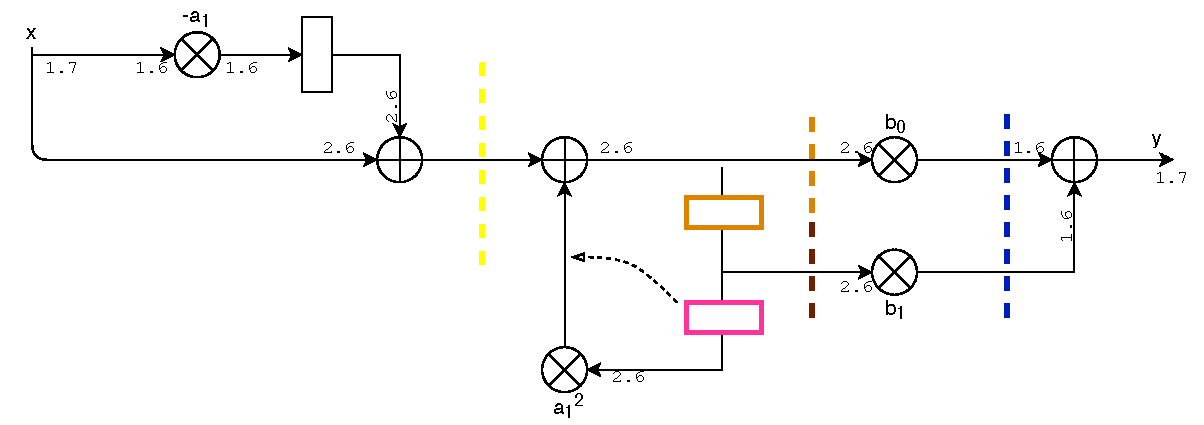
\includegraphics[width=1.2\textwidth]{./chapter3/images/fastdfg_inter.pdf}}
	\caption{Initial DFG with annotated parallelism. Dashed vertical lines indicate cutsets where pipeline stages will be inserted. The pink register 
		can be moved to the position indicated by the arrow by means of retiming}
	\label{fig:fast_dfg_inter}
\end{figure}

\begin{figure}
	\makebox[\textwidth][c]{
	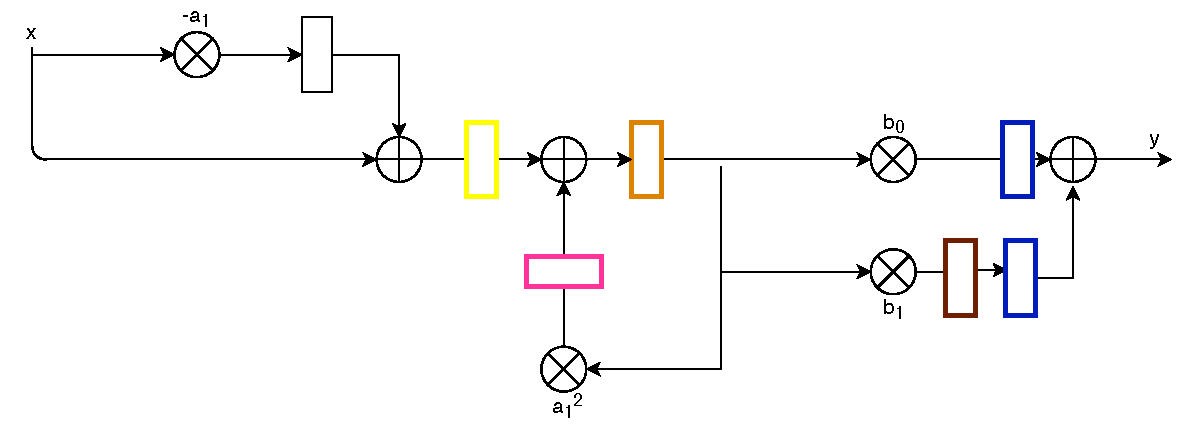
\includegraphics[width=1.2\textwidth]{./chapter3/images/fastdfg_final.pdf}}
	\caption{Final DFG. Colors identify registers corresponding to the DFG in figure \autoref{fig:fast_dfg_inter}}
	\label{fig:fast_dfg_final}
\end{figure}

\section{Control Unit}
The addition of pipeline stages increases dramatically the number of possible states in our FSM, making it impractical to describe the control unit by enumerating all of them. We resorted to a structural description consisting of a delay line where a number of flip-flops are connected in cascade. The delay line contains two flip flops plus one additional flip flop for each pipeline stage, which amounts to a total of five delay units. One additional register samples the reset signal and controls \texttt{clear\_w\_regs}, a signal that causes the unit to enter the reset state for a single clock cycle, where both the datapath registers and the delay line are cleared. The latch enable signal is found at the output of the first flip flop, whereas VOUT corresponds to the end of the delay line.
